\documentclass{beamer}
\usepackage{beamerthemeshadow}
\beamertemplatetransparentcovereddynamic
\usepackage{graphicx}
\usepackage{amsmath}
\usepackage{algorithm}
\usepackage{algorithmic}
\usepackage{psfrag}

%PSO Stuff
\DeclareMathOperator{\URand}{U}
\providecommand{\ppos}{\ensuremath{\Vec{x}}}
\providecommand{\pvel}{\ensuremath{\Vec{v}}}
\providecommand{\nbest}{\ensuremath{\Vec{b}_n}}
\providecommand{\pbest}{\ensuremath{\Vec{b}_p}}
\providecommand{\constriction}{\ensuremath{\chi}}
\providecommand{\coeff}{\ensuremath{\phi}}
\providecommand{\nURand}{\ensuremath{U^\neigh}}
\providecommand{\pURand}{\ensuremath{U^\pers}}
\providecommand{\ncoeff}{\ensuremath{\phi^\neigh}}
\providecommand{\pcoeff}{\ensuremath{\phi^\pers}}
\providecommand{\pers}{\ensuremath{P}}
\providecommand{\neigh}{\ensuremath{N}}

%SpecExPSO Stuff
\providecommand{\noeval}[1]{\ensuremath{#1^{-e}}}
\providecommand{\nonbest}[1]{\ensuremath{#1^{-n}}}
\providecommand{\p}{\ensuremath{p}}
\providecommand{\pset}{\ensuremath{\mathbf{p}}}
\providecommand{\s}{\ensuremath{s}}
\providecommand{\sset}{\ensuremath{\mathbf{s}}}
\providecommand{\nsset}{\ensuremath{\mathbf{ns}}}
\providecommand{\n}{\ensuremath{n}}
\providecommand{\nset}{\ensuremath{\mathbf{n}}}
\providecommand{\nnset}{\ensuremath{\mathbf{nn}}}
\providecommand{\leftnbold}{\ensuremath{\Vec{\mathbf{x}}^\mathbf{\leftind}}}
\providecommand{\rightnbold}{\ensuremath{\Vec{\mathbf{x}}^\mathbf{\rightind}}}
\providecommand{\nbestbold}{\ensuremath{\Vec{\mathbf{x}}^\mathbf{\neigh}}}
\providecommand{\pbestbold}{\ensuremath{\Vec{\mathbf{x}}^\mathbf{\pers}}}
\providecommand{\pposbold}{\ensuremath{\Vec{\mathbf{x}}}}
\providecommand{\leftn}{\ensuremath{\Vec{x}^\leftind}}
\providecommand{\rightn}{\ensuremath{\Vec{x}^\rightind}}
\providecommand{\leftind}{\ensuremath{L}}
\providecommand{\rightind}{\ensuremath{R}}
\providecommand{\casexn}{\ensuremath{(S,-)}}
\providecommand{\casexx}{\ensuremath{(S,S)}}
\providecommand{\casexl}{\ensuremath{(S,\leftind)}}
\providecommand{\casexr}{\ensuremath{(S,\rightind)}}
\providecommand{\casepn}{\ensuremath{(-,-)}}
\providecommand{\casepl}{\ensuremath{(-,\leftind)}}
\providecommand{\casepr}{\ensuremath{(-,\rightind)}}
\providecommand{\casepN}{\ensuremath{(-,N)}}
\providecommand{\casexN}{\ensuremath{(S,N)}}

\psfrag{equation 1}{$\ppos_{t-1} +
  \constriction \bigl[ \pvel_{t-1} +
	\pcoeff\pURand_{t-1}\otimes(\pbestbold_{\mathbf{t-1}} - \ppos_{t-1}) + 
	\ncoeff\nURand_{t-1}\otimes(\nbestbold_{\mathbf{t-1}} - \ppos_{t-1})
  \bigr]$
}
\psfrag{equation --}{$\ppos_{t} +
  \constriction \bigl[ \pvel_{t} +
	\pcoeff\pURand_{t}\otimes(\pbestbold_{\mathbf{t-1}} - \ppos_{t}) + 
	\ncoeff\nURand_{t}\otimes(\nbestbold_{\mathbf{t-1}} - \ppos_{t})
  \bigr]$
}
\psfrag{equation -l}{$\ppos_{t} +
  \constriction \bigl[ \pvel_{t} +
	\pcoeff\pURand_{t}\otimes(\pbestbold_{\mathbf{t-1}} - \ppos_{t}) + 
	\ncoeff\nURand_{t}\otimes(\leftnbold_{\mathbf{t}} - \ppos_{t})
  \bigr]$
}
\psfrag{equation -r}{$\ppos_{t} +
  \constriction \bigl[ \pvel_{t} +
	\pcoeff\pURand_{t}\otimes(\pbestbold_{\mathbf{t-1}} - \ppos_{t}) + 
	\ncoeff\nURand_{t}\otimes(\rightnbold_{\mathbf{t}} - \ppos_{t})
  \bigr]$
}
\psfrag{equation s-}{$\ppos_{t} +
  \constriction \bigl[ \pvel_{t} +
	\pcoeff\pURand_{t}\otimes(\pposbold_{\mathbf{t}} - \ppos_{t}) + 
	\ncoeff\nURand_{t}\otimes(\nbestbold_{\mathbf{t-1}} - \ppos_{t})
  \bigr]$
}
\psfrag{equation sl}{$\ppos_{t} +
  \constriction \bigl[ \pvel_{t} +
	\pcoeff\pURand_{t}\otimes(\pposbold_{\mathbf{t}} - \ppos_{t}) + 
	\ncoeff\nURand_{t}\otimes(\leftnbold_{\mathbf{t}} - \ppos_{t})
  \bigr]$
}
\psfrag{equation sr}{$\ppos_{t} +
  \constriction \bigl[ \pvel_{t} +
	\pcoeff\pURand_{t}\otimes(\pposbold_{\mathbf{t}} - \ppos_{t}) + 
	\ncoeff\nURand_{t}\otimes(\rightnbold_{\mathbf{t}} - \ppos_{t})
  \bigr]$
}
\psfrag{equation ss}{$\ppos_{t} +
  \constriction \bigl[ \pvel_{t} +
	\pcoeff\pURand_{t}\otimes(\pposbold_{\mathbf{t}} - \ppos_{t}) + 
	\ncoeff\nURand_{t}\otimes(\pposbold_{\mathbf{t}} - \ppos_{t})
  \bigr]$
}
\title[A Speculative Approach to Parallelization in PSO]{A Speculative Approach
to Parallelization in Particle Swarm Optimization}
\author{Matthew Gardner}
\date{\today}

\begin{document}
\begin{frame}
  \titlepage
\end{frame}

\begin{frame}
  \frametitle{Thesis Statement}
When many processors are available, a speculative approach to the
parallelization of PSO can yield dramatic improvements in the performance of
the algorithm on expensive functions compared to previous parallelization
techniques.
\end{frame}

\section{Particle Swarm Optimization}
\begin{frame}
  \frametitle{Optimization}
  \includegraphics[width=\textwidth]{cosine}
\end{frame}

\subsection{Basic Idea}
\begin{frame}
  \frametitle{Particle Swarm Optimization}
  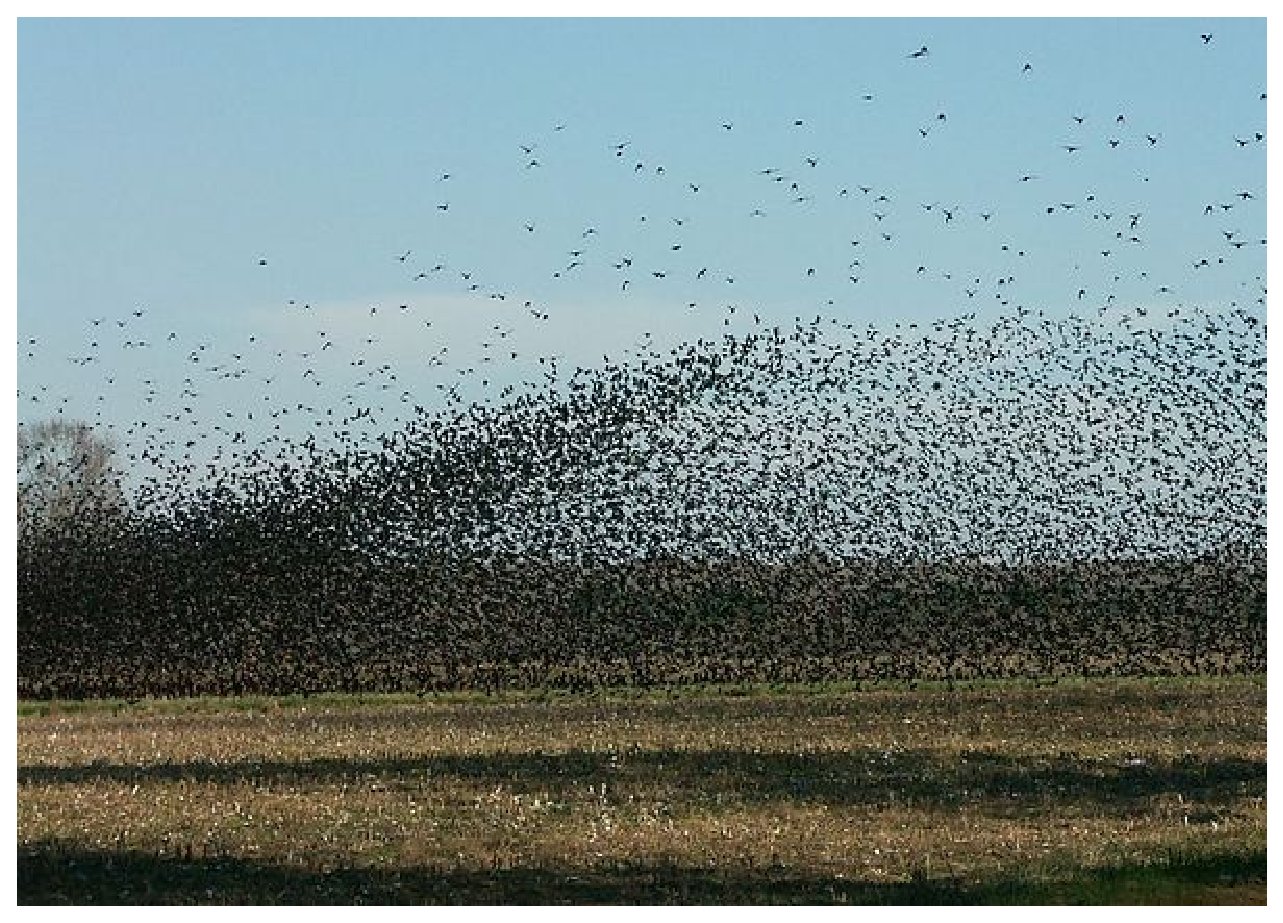
\includegraphics[width=\textwidth]{birds}
\end{frame}

\subsection{The Math}
\begin{frame}
  \frametitle{PSO Equations}
  \begin{align*}
	  \pvel_{t+1} &=
		  \constriction \left[ \pvel_t +
			  \coeff_1\URand()\otimes(\pbest - \ppos_t) +
			  \coeff_2\URand()\otimes(\nbest - \ppos_t)
		  \right] \\
	  \ppos_{t+1} &= \ppos_t + \pvel_{t+1}
  \end{align*}
\end{frame}

\section{Speculative Evaluation}

\subsection{Speculative Execution}
\begin{frame}
  \frametitle{Speculative Execution}
  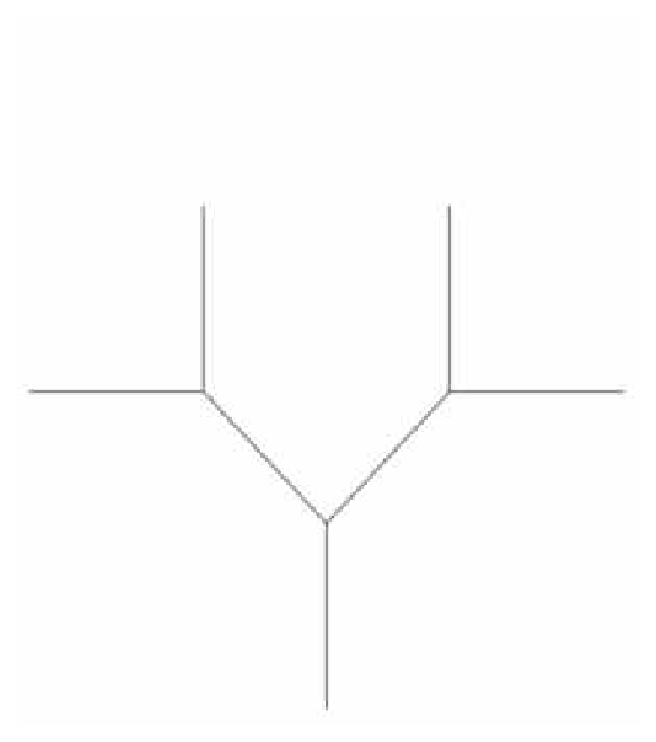
\includegraphics[width=\textwidth]{branching}
\end{frame}

\subsection{Speculative Evaluation in PSO}
\begin{frame}
  \frametitle{Speculative Evaluation in PSO}
  \begin{align*}
	  \pvel_{t+1} &=
		  \constriction \left[ \pvel_t +
			  \coeff_1\URand()\otimes(\pbest - \ppos_t) +
			  \coeff_2\URand()\otimes(\nbest - \ppos_t)
		  \right]
  \end{align*}
  \pause
  \begin{center}
	\begin{tabular}{lcc}
	  Identifier&Source of $\pbest$ update&Source of $\nbest$ update\\
	  \hline
	  \hline
	  $\casepn$&No update&No update\\
	  \hline
	  $\casexn$&Self&No update\\
	  \hline
	  $\casexx$&Self&Self\\
	  \hline
	  $\casepl$&No update&Left Neighbor\\
	  \hline
	  $\casexl$&Self&Left Neighbor\\
	  \hline
	  $\casepr$&No update&Right Neighbor\\
	  \hline
	  $\casexr$&Self&Right Neighbor\\
	  \hline
	\end{tabular}
  \end{center}
\end{frame}

\subsection{Relaxations}

\begin{frame}
  \frametitle{Branch Pruning}
  \includegraphics[height=.8\textheight]{speculative_evaluation}
\end{frame}

\begin{frame}
  \frametitle{Branch Pruning}
  \includegraphics[height=.8\textheight]{pruning}
\end{frame}

\begin{frame}
  \frametitle{Several Iterations Ahead}
  \includegraphics[width=\textwidth]{manyiters}
\end{frame}

\end{document}
